% Made up for the tikra benchmark.
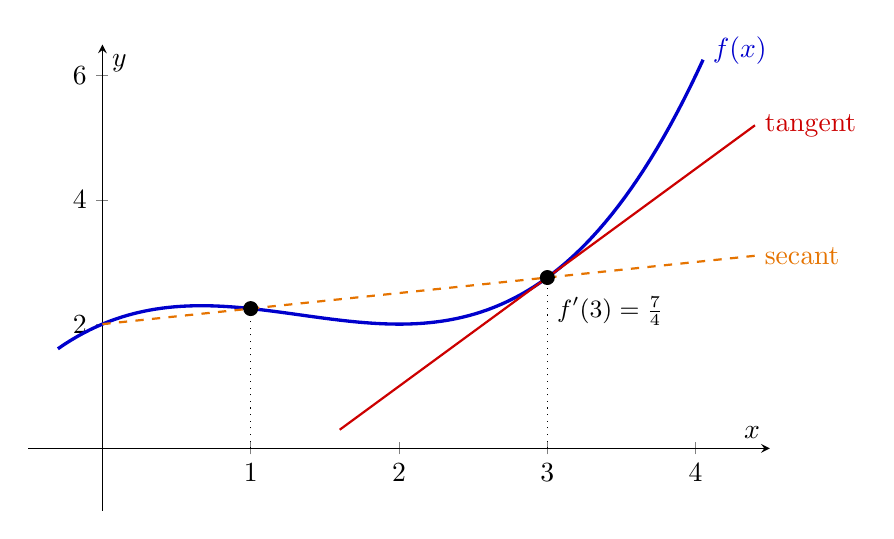
\begin{tikzpicture}
\begin{axis}[width=11cm, height=7.5cm, axis lines=middle, xmin=-0.5, xmax=4.5, ymin=-1, ymax=6.5,
    xlabel=$x$, ylabel=$y$, xtick={1,2,3,4}, ytick={2,4,6}, domain=-0.3:4.05, samples=100,
    clip=false]
  \addplot[very thick, blue!80!black] {0.25*x^3 - x^2 + x + 2};
  \node[blue!80!black, anchor=west] at (axis cs:4.05,6.4) {$f(x)$};
  % tangent at x = 3: f(3) = 2.75, f'(3) = 1.75
  \addplot[thick, red!80!black, domain=1.6:4.4] {2.75 + 1.75*(x-3)};
  \node[red!80!black, anchor=west] at (axis cs:4.4,5.2) {tangent};
  % secant through x = 1 and x = 3: f(1) = 2.25
  \addplot[thick, dashed, orange!90!black, domain=0:4.4] {2.25 + 0.25*(x-1)};
  \node[orange!90!black, anchor=west] at (axis cs:4.4,3.1) {secant};
  \addplot[only marks, mark=*, mark size=2.5pt, black] coordinates {(1,2.25) (3,2.75)};
  \draw[dotted] (axis cs:3,0) -- (axis cs:3,2.75);
  \draw[dotted] (axis cs:1,0) -- (axis cs:1,2.25);
  \node[anchor=north west, font=\small] at (axis cs:3,2.6) {$f'(3) = \frac{7}{4}$};
\end{axis}
\end{tikzpicture}
